\documentclass[12pt]{article}
\usepackage[frenchb]{babel}
\usepackage{fontenc}
\usepackage{fancyhdr} % Required for custom headers
\usepackage{lastpage} % Required to determine the last page for the footer
\usepackage{extramarks} % Required for headers and footers
\usepackage{graphicx} % Required to insert images
\usepackage[utf8]{inputenc}
\usepackage{url}
\usepackage[normalem]{ulem}
\usepackage{geometry}
\usepackage{listings}
\usepackage{numprint}
\usepackage{eurosym}
\usepackage{appendix}
\usepackage{pdfpages}

\geometry{a4paper,
		  body={160mm,250mm},
		  left=20mm,
		  top=25mm,
		  bottom=25mm,
		  right=15mm,
		  headheight=10mm,
		  headsep=4mm,
		  marginparsep=4mm,
		  marginparwidth=21mm}
		  
\pagestyle{fancy}
\lhead{\Right}
\rhead{\ \thepage}
\lfoot{\lastxmark}
\cfoot{Lucie Herrier 3TL1}
\rfoot{}
\renewcommand\headrulewidth{0.4pt} % Size of the header rule
\renewcommand\footrulewidth{0.4pt} % Size of the footer rule

\newcommand{\ephec}{
\includegraphics[width=2cm]{ephec.png}}
\newcommand{\Right}{Une application Android au service de l'apprentissage de la lecture chez l'enfant}

\begin{document}
\title{
\parbox{15cm}
{	
	\begin{center}
	\large ECOLE PRATIQUE DES HAUTES ETUDES COMMERCIALES\\
	\vspace{.5cm}
	
\includegraphics[width=5cm]{ephec.png}\\
	Avenue du Ciseau 15\\
	1348 Louvain-La-Neuve\\
	\vspace{2cm}
	\sf\bfseries\Huge
	Une application android au service de l'apprentissage de la lecture chez l'enfant 
	\rule{15cm}{1pt}\\
	\normalsize\mdseries Travail de fin d'études présenté en vue de l'obtention du diplôme de bachelier en Informatique et Systèmes : finalité Technologie de l'Informatique\\
	\vspace{1cm}
	Future image\\
	%\includegraphics[width=5cm]{Onetec1.png}\\
	\vspace{.5cm}
	\bfseries\LARGE
		Lucie HERRIER\\ \Large 3TL1
	\rule{15cm}{1pt}
	\end{center}
	\vspace{1cm}
	\bf\normalsize Rapporteur : Virginie VAN DEN SCHRIECK
	\vspace{4cm}
	\begin{center}
	\Large Année Académique 2014-2015
	\end{center}
}} 

\thispagestyle{empty}
\date{}
\maketitle
\thispagestyle{empty}
\newpage
\vspace*{\stretch{1}}
\begin{center}
\begin{minipage}{0.8\textwidth}
\textit{Je voudrais remercier plusieurs personnes pour leur aide à la réalisation de ce travail de fin d'études. Tout d'abord Mme Van den Schrieck, pour m'avoir mis en contact avec l'école des Bruyères, et son feedback sur mon travail. Je remercie également Odile Paveau, institutrice à l'école primaire des Bruyères, ainsi que Laurence Henrion, pour m'avoir expliqué les méthodes d'apprentissage de la lecture chez les enfants, [ETC].\\
Par ailleurs, je remercie l'équipe enseignante de la section Technologie de l'Informatique de l'EPHEC LLN, sans laquelle je n'aurais pas pu acquérir les compétences nécessaires à la réalisation de ce travail.\\
Enfin, merci à tous ceux que j'aurais oublié, et qui m'ont d'une manière ou d'une autre aidé et soutenu dans le cadre de ce TFE. }
\end{minipage}
\end{center}
\vspace*{\stretch{1}}

\thispagestyle{empty}
\newpage
\pagenumbering{Roman}
\setcounter{page}{1}
\tableofcontents
\newpage
\pagenumbering{arabic}
\setcounter{page}{1}
\section{Introduction : Énoncé de la thématique du TFE et motivations}
Le rôle des nouvelles technologies dans l'apprentissage chez les enfants est un sujet qui m'intéresse tout particulièrement. Je me suis souvent interrogée sur les bienfaits, ou méfaits selon certains, de l'utilisation d'appareils informatiques chez les plus jeune. De ce fait, j'ai décidé de consacrer mon travail de fin d'études au développement d'une application android afin d'aider et complémenter l'apprentissage de la lecture chez les enfants, en parallèle à l'école. La programmation android est d'autant plus actuelle que le nombre de tablettes et de smartphones est en constante augmentation, et que la majorité de ces appareils tournent sous le célèbre système d'exploitation de Google. La pertinence de cette problématique s'est d'ailleurs confirmée au cours des travaux préparatoires de ce travail de fin d'études : parmi les applications disponibles, peu d'entre elles ont été réalisées en se basant sur les précieux conseils de professionnels du secteur de l'apprentissage.\\

Ce travail de développement d'application s'appuie essentiellement sur l'analyse des informations obtenues auprès d'une institutrice, d'une logopède, et même de l'avis des enfants. Intitulé "Une application android au service de l'apprentissage de la lecture chez l'enfant ", ce travail de fin d'étude tend à démontrer qu'il est possible qu'android aide les enfants à apprendre, conjointement à la méthode traditionnelle employée par les instituteurs. En effet, un application peut entraîner les enfants dans l'apprentissage de la lecture, tout en s'amusant.\\

Après une première partie consacrée à la recherche documentaire, où l'on observe que j'y expose ce que j'ai appris lors de mes entretiens avec les personnes travaillant dans le domaine de l'apprentissage de la lecture chez l'enfant, le point suivant est consacré à une présentation de l'application ainsi que des exercices qui s'y retrouven. Celui-ci explique les choix auxquels j'ai procédé afin de mettre en place des exercices reflétant au mieux les conseils obtenus précédemment. Par la suite, je présente les outils et technologies que j'ai utilisés afin de mener à bien ce projet, avant d'expliciter la manière dont s'est déroulé le développement android à proprement parler. Enfin, je termine ce rapport par une analyse des difficultés que j'ai pu rencontrer tout au long de ce travail de fin d'études, ainsi que les améliorations qu'il serait possible d'apporter à l'application android, avant de conclure.
%\section{Présentation de l'application}

\section{Analyse du problème}
Avant de me lancer dans la partie technique et la programmation de ce travail de fin d'études, il m'a fallu effectuer quelques recherches. En effet, ne s'improvise pas instituteur qui veut. Bien que nous ayons tous dans notre vie appris à lire, il m'était impossible d'imaginer concevoir sans aucune aide une application supposée aider les enfants dans leur apprentissage de la lecture. J'ai donc choisi de me documenter auprès de professionnelles travaillant avec des enfants. Afin de valider la pertinence de la problématique, je me suis également renseignée sur les applications existantes, tout en recoupant leur contenu avec les informations obtenues précédemment.\\

Ce point est consacré aux recherches que j'ai effectuées avant de commencer l'application en elle-même. Je présenterai tout d'abord les informations obtenues auprès de l'institutrice et de la logopède, ainsi que la conclusion de ces deux entrevues. J'analyserai ensuite les produits existants sur le marché sur la base des informations obtenues. Je terminerai avec le cahier des charges établi pour l'application suite à ces recherches.

\subsection{Rencontre avec des professionnelles de l'apprentissage de la lecture}
J'ai choisi de commencer mon travail par une étape de documentation auprès de professionnelles travaillant avec des enfants. Pour ce faire, j'ai eu recours à l'aide et l'expérience de Mme Odile Paveau, institutrice primaire à l'école des Bruyères de Louvain-La-Neuve, ainsi que de Mme Laurence Henrion, logopède exerçant à Louvain-La-Neuve également. Toutes deux m'ont dit être intéressées par le sujet de mon TFE. Elle ont accepté de me fournir des explications, des conseils, et des pistes pour le bon développement de mon application Android. Ci-dessous se trouvent les synthèses des entrevues; le compte-rendu complet des rencontres figure quant à lui dans l'annexe \ref{annexeInterview}.

\subsubsection{Rencontre avec une institutrice : Odile Paveau\label{Freinet}}
J'ai rencontré Odile Paveau le 16 décembre 2014 dans la classe de primaire où elle enseigne, à l'école des Bruyères de Louvain-La-Neuve. Lors de cette entrevue, trois grands points ont été abordés : les méthodes d'apprentissage les plus utilisées pour la lecture, les spécificités de l'apprentissage à l'école des Bruyères, et la présentation d'outils utilisés ainsi que des exemples d'exercices.\\

Il existe bon nombre de méthodes d'apprentissage, qui peuvent être très variées. Parmi celles-ci, Odile a fait mention de trois méthodes en particulier, et qui concernent l'apprentissage de la lecture :
\begin{itemize}
\item la méthode globale,
\item la méthode syllabique,
\item la méthode naturelle.\\
\end{itemize} 

La méthode globale consiste à apprendre à lire à partir du mot en entier. Le but de cette méthode est \textit{"de faire acquérir à l'élève une stratégie de déchiffrage des mots, voire des phrases, en tant qu'image visuelle indivisible"}\footnote{Citation tirée de l'article \textit{Méthode globale}, http://fr.wikipedia.org/wiki/Méthode\_globale}. En pratique, cela signifie que l'enfant, la première fois qu'il rencontre le mot, est invité à le deviner. Celui-ci mémorisera alors le mot en le rencontrant plusieurs fois dans des contextes différents (chansons, petites histoires, poèmes, ...). Le mot est dès lors associé à une idée, ce qui permet de qualifier cette méthode d'\textit{idéovisuelle}.\\

La méthode syllabique, par opposition à la méthode globale, part des sons que forment les lettres et les syllabes afin de construire le mot. Celle-ci relie la phonétique des lettres avec l'alphabet afin de construire tout d'abord les syllabes, puis d'assembler ces dernières pour créer les mots. Cette méthode se base sur le décryptage progressif des phrases lues.\\

La méthode naturelle s'inspire quant à elle de la pédagogie Freinet. Cette dernière, mise au point par Célestin Freinet au siècle dernier, est fondée sur l'expression de la créativité des enfants. Il s'agit de donner à l'enfant un projet, qui lui sera utile dans son apprentissage, et qui prend en compte ses centres d'intérêts et le potentiel créatif et associatif de celui-ci. Du point de vue de l'apprentissage de la lecture, cette méthode implique de partir du sens des mots, afin de donner un sens à ce qui est appris. La collaboration de tout le groupe est nécessaire, et l'essai-erreur est appliqué. La pédagogie Freinet a d'abord été associée à la méthode globale. Cependant, son procédé différant dans la façon dont les mots sont appris, l'apprentissage de la lecture par cette pédagogie se nomme désormais méthode naturelle.\\

A l'école des Bruyères, les instituteurs ne se concentrent pas sur une méthode en particulier pour enseigner la lecture aux enfants. Ce sont les méthodes syllabique, pour son apprentissage fluide, et naturelle qui sont principalement utilisées, comparativement à "l'ancienne technique" des écoles primaire, dans laquelle la méthode globale primait. Néanmoins, la méthode globale n'est pas totalement remisée au placard, car elle est encore d'application dans certains exercices. Elle reste cependant peu utilisée, étant considérée comme lourde et peu optimale, à contrario des deux autres qui peuvent être plus ludiques. En effet, il est très important de faire sens pour l'enfant et de susciter son intérêt afin de faciliter l'apprentissage.\\

Pour apprendre à lire et mettre en pratique ces méthodes, les enfants utilisent divers outils. Tout d'abord, notons que la lecture s'apprend en premier lieu à l'aide de caractères imprimés en majuscules, puis en minuscules, et enfin avec la police de type écriture manuelle, appelée aussi \textit{cursive}. Ceci permet aux enfants de se familiariser petit à petit avec les lettres, celles-ci présentant des motifs plus complexes au fil des étapes. Ensuite, l'enfant travaille beaucoup sur ses centres d'intérêts. Il faut le faire travailler sur des sujets qui le concernent ou l'amusent tels que son prénom, son âge, ce qu'il aime, des phrases rigolotes, etc.\\

Durant l'apprentissage, le rapport au son est très important pour l'enfant. Voici quelques exercices et outils qui sont proposés à l'école :
\begin{itemize}
\item Avec des lettres d'imprimerie disposées dans n'importe quel sens\footnote{Le fait de mettre les lettres droites, à l'envers, ou de côté permet d'entraîner l'enfant à différencier les caractères.}, l'institutrice donne un son, et il faut retrouver la lettre qui produit ce son.
\item Classer les prénoms des enfants de la classe en les rassemblant en fonction des sons par lesquels ils commencent. Ceci permet notamment de découvrir de nouveau phonèmes, comme dans le prénom \textit{Hugo}, où le son entendu est \textit{U} et le phonème associé est \textit{Hu}.
\item Dans un petit texte, qui peut être écrit sur la base d'une idée de l'enfant (par exemple "\textit{Marie aime la danse et les poupées}"), retrouver les sons déjà connus et les souligner en couleur. La couleur aide ici et à mémoriser, et à différencier.
\item Dans un texte, trouver le son qui revient le plus souvent. Cet exercice est une variante du précédent.
\item A partir d'un son, trouver des mots qui commencent par celui-ci, par exemple sous forme d'images pour ensuite voir comment s'écrit le mot. Au niveau supérieur, le son peut se trouver au milieu ou en fin de mot.
\item Comme outil, créer un dictionnaire \textit{référent}. Celui-ci reprend, pour chaque son (également les composés type \textit{au, ou, en, ...}) un dessin représentatif du son (par exemple une chouette pour le son \textit{ch}) ainsi qu'une liste des mots commençant par ce son.
\item Retrouver un mot connu dans un texte (ici, la méthode globale est utilisée).
\item Etc.\\
\end{itemize}

Lors des évaluations de l'apprentissage de la classe, la méthode naturelle est la plus souvent utilisée, car c'est celle qui fait le plus appel à l'imagination de l'enfant. Comme outil, les instituteurs utilisent notamment les fichiers Freinet. Créés sur base de la pédagogie Freinet, ces fichiers sont composés d'images associées à des mots de différents niveaux. L'idée est d'associer un (ou plusieurs) mot(s) lu(s) à une (ou plusieurs) image(s), et de vérifier les capacités de lecture de l'enfant en lui proposant soit le même mot à retrouver dans une liste sur base d'une image semblable à la précédente, soit un mot différent sur base d'une image différente des deux précédentes, soit encore l'association d'un nouveau mot en complément avec celui lu précédemment, sous forme d'une phrase. Des exemples de fichiers se trouvent à l'annexe \ref{annexeFreinet}. Ces fichiers existent également pour d'autres matières, comme les mathématiques.\\

Enfin, à l'école des Bruyères, l'enfant à toujours accès à une boîte à outils pour s'aider en cas de difficultés. Celle-ci est composée du dictionnaire référent, mais aussi de panneaux et d'affiches se trouvant un peu partout dans la classe. Ceux-ci rappellent les couleurs identifiants les sons, les images associées, les dessins des enfants représentant des mots, des symboles associés aux lettres, etc.

\subsubsection{Rencontre avec une logopède : Laurence Henrion}
J'ai rencontré Laurence Henrion le 19 janvier 2015. Elle a accepté de me recevoir dans le cabinet où elle exerce son activité de logopède. Durant notre entrevue, elle a mentionné différents points que je considère comme importants, et que je détaillerai ci-dessous : l'importance de l'âge et les connaissances de bases pour la lecture, les exercices qu'elle utilise en tant que logopède et les applications spécialisées, et enfin les détails pratiques pouvant m'aider pour la programmation de mon application.\\

Comme expliqué précédemment, il existe plusieurs méthodes pour apprendre à l'enfant à lire. L'idéal, cependant, est de commencer à lui inculquer les bases de la lecture vers 3 ou 4 ans. En effet, ceci permet d'optimiser ses compétences par la suite. Ce principe vient notamment des méthodes pédagogiques proposées par Maria Montessori\footnote{Pour plus d'informations : \textit{Pédagogie Montessori}, \url{http://fr.wikipedia.org/wiki/Pédagogie_Montessori}}. Cette pédagogie met l'accent sur l'importance des périodes sensibles de l'enfant\footnote{Une période sensible est un âge où l'enfant est plus prompt à développer certains aspect de son évolution naturellement.}. Celle concernant le langage se déroule environ de 2 mois à 6 ans. La pédagogie Montessori part du principe qu'il existe une conscience phonologique fort présente chez l'enfant à ce moment. Celui-ci apprend beaucoup à l'aide de rimes, de comptines, etc. C'est-à-dire à l'aide de sons. Ceci rejoint ce qui m'avait déjà été dit par Odile à propos de la méthode syllabique : il est important de se baser sur le son que fait la lettre seule, ou le groupe de lettres, et non le nom qui lui est donné, car ce dernier est source de confusions.\\

Néanmoins, être dans la bonne période ne suffit pas pour maîtriser l'art de la lecture. En effet, pour apprendre à lire, l'enfant doit déjà maîtriser un certain vocabulaire à l'oral. Dès lors, si le vocabulaire de base n'est pas acquis, l'enfant ne sera pas capable de comprendre ce qu'il lit. Les premiers mots et textes seront dont composés de vocabulaire basique, pas de mots compliqués et peu fréquents, tels que \textit{narval}, \textit{okapi}, etc.\\

En tant que logopède, Laurence Henrion travaille avec différents exercices basés sur le son. Certains exercices rejoignent ce qui avait été dit aux Bruyères, notamment :
\begin{itemize}
\item La sélection d'un mot contenant un son entendu précédemment parmi plusieurs choix.
\item Choisir une lettre qui produit le son prononcé. Ici, Laurence Henrion m'a spécifié que la lettre importait peu tant que le son était correct. Par exemple, pour le son \textit{sss}, l'enfant peut choisir aussi bien le \textit{s} que le \textit{c} ou le \textit{ç.}
\item Relier un mot ou un son à une image.
\item Associer les sons et les lettres à des couleurs qui leur seront spécifiques.\\
\end{itemize}

Un autre exercice qu'elle affectionne particulièrement est la lecture flash.
Cet exercice consiste à mémoriser un mot (ou une phrase) affiché plus ou moins rapidement à l'écran, pour ensuite le réécrire correctement. Dans le cas présent, l'orthographe est travaillée en plus de la lecture. Ce sont deux matières très liées. Un jeu de lecture flash doit idéalement :
\begin{itemize}
\item avoir un temps réglable d'affichage selon le niveau de l'enfant,
\item insister sur l'importance de la mémorisation,
\item faire attention au sens de la lecture.
\end{itemize}
En plus de cela, l'exercice peut être amélioré grâce à :
\begin{itemize}
\item l'affichage de mots personnalisés en fonction des centres d'intérêt de l'enfant,
\item la lecture effectuée avec un mot, et la réécriture sous la forme d'une image à choisir.\\
\end{itemize}

Laurence Henrion utilise beaucoup son iPad pour travailler avec les enfants. En effet, c'est plus fun pour l'enfant de jouer avec une tablette.
La majorité des applications présentes sur l'iPad ont été créés par un spécialiste orthophoniste (appelation d'un logopède en France) : Emmanuel Crombez. Celui-ci réalise des applications pour iPad, iPhone et Mac sous le nom \textit{ABC Applications}. Celles-ci sont destinées à aider les enfants dans leur apprentissage général et dans leurs difficultés : lecture, écriture, mathématiques, etc. Parmi ces jeux, on peut trouver\footnote{Liste complète sur le site d'Emmanuel Crombez : \url{http://abc-applications.com/ipad.html}.} :
\begin{itemize}
\item \textit{Anagrammes}. L'enfant doit retrouver des mots dont les lettres ont été mélangées. Au besoin, il peut s'aider en écoutant le mot qu'il doit reconstituer.
\item \textit{Nuages de mots}. Cet exercice propose à l'enfant de retrouver le genre et le nombre des mots affichés en "nuages". Quel mot est masculin, ou féminin ? Est-ce singulier ou pluriel ? Le jeu entraîne à la lecture mais aussi au classement. Ce jeu existe aussi sous la forme \textit{Nuages de lettres}, adapté aux enfants de maternelle pour apprendre à reconnaître les lettres.
\item \textit{Mémo des mots}. Ce jeu se présente sous la forme du bien connu \textit{Memory}. La différence étant qu'ici des mots sont utilisés à la place des images.
\textit{Etc.}\\
\end{itemize}

Pour terminer, j'ai reçu quelques conseils concernant ce qui était préférable d'éviter pour mon application, et ce qui pouvait m'être utile. Tout d'abord, il est déconseillé d'inclure trop d'éléments graphiques. Il vaut mieux opter pour un design simple et épuré. Trop d'objets sur l'écran, c'est prendre le risque que l'enfant soit distrait et ne se concentre pas sur ce qui est requis, donc perdre en efficacité. Ensuite, il existe une police open source conçue pour faciliter la lecture chez les personnes dyslexiques en accentuant certaines parties des lettres. Celle-ci se nomme \textit{OpenDyslexic}. Dans le cas où celle-ci n'aurait pas été disponible, un police de type sans serif telle que \textit{Verdana} est idéale. En dernier lieu, Laurence m'a conseillé d'utiliser le VOB (Vocabulaire Orthographique de Base) pour les exercices que je mettrais en place dans l'application. Il s'agit de la liste officielle en Belgique des mots qui doivent être connus et maîtrisés par les enfants à la fin de chaque cycle de primaire.

\subsection{Conclusion des entrevues}
Les interviews avec Odile Paveau et Laurence Henrion m'ont permis de comprendre les méthodes utilisées dans l'apprentissage de la lecture chez l'enfant. Elles m'ont expliqué ce qui était le plus efficace, ainsi que les erreurs que je devais éviter. Voici ce que j'en ai retiré.\\

Premièrement, je me suis renseignée un peu plus sur les différentes méthodes d'apprentissage afin de choisir ce que j'allais développer comme exercices. Je n'ai pas étudié le sujet en profondeur, l'essentiel pour moi étant de bien comprendre le fonctionnement des méthodes et ce que je pouvais en retirer. Voici en quelques mots une synthèse des différentes méthodes et pédagogies qui ont été abordées :
\begin{itemize}
\item la méthode globale : apprendre à lire à partir du mot en entier. C'est une méthode idéovisuelle qui veut que l'enfant mémorise les mots rencontrés sous forme d'image et d'idée, et puisse les reconnaître plus tard;
\item la méthode syllabique : opposée à la méthode globale, elle part du son des syllabes et des lettres pour former les mots. Il s'agit ici de déchiffrer;
\item la méthode naturelle inspirée de la pédagogie Freinet : elle part du sens des mots et des intérêts de l'enfant. L'idée est de stimuler l'enfant, sa créativité, ce qu'il aime, afin de mémoriser le mot;
\item la pédagogie Montessori : met l'accent sur les périodes sensibles de l'enfant et l'apprentissage spécifique lié à celles-ci. Pour la période liée au langage et à la lecture, il existe une conscience phonologique fort présente chez l'enfant : il apprend beaucoup grâce aux comptines, chansons, rimes, etc.
\end{itemize}
Tant Odile que Laurence ont insisté sur l'intérêt que doit porter l'enfant aux jeux et exercices, ainsi que sur l'efficacité de travailler avec les sons des lettres et les syllabes. Il est donc évident pour moi que les méthodes idéales pour une application sont la méthode syllabique et la méthode naturelle. Concernant la pédagogie Montessori, je n'ai pas de prise sur l'âge des utilisateurs.\\

À côté des méthodes d'apprentissage, différents éléments ressortent des entrevues. Tout d'abord, le point le plus important est de susciter l'intérêt de l'enfant pour l'apprentissage de la lecture. Éveiller sa curiosité en choisissant des sujets qui l'intéressent ou en utilisant des exercices ludiques lui permet d'apprendre plus efficacement.\\

D'autre part, certains exercices m'ont paru plus importants, ou plus intéressants comparés à d'autres. Le premier est celui où il faut retrouver les sons de lettres ou de syllabes dans les mots. Autant Odile que Laurence m'en ont parlé comme d'une "base" dont l'efficacité a été prouvée.
Certains des autres exercices mentionnés me paraissent également adaptables pour mon application :
\begin{itemize}
\item les fichiers Freinet pour la lecture,
\item retrouver des mots dans un texte,
\item la lecture flash, sur laquelle Laurence Henrion a particulièrement insisté,
\item les anagrammes,
\item les nuages de mots.\\
\end{itemize}

Enfin, le dernier point, très important à mes yeux, est le conseil d'utilisation de la police spécialisée \textit{OpenDyslexic} pour la lisibilité du texte de l'application, ainsi que l'emploi du VOB pour le vocabulaire proposé.

\subsection{Étude des produits existants et critique sur la base des entrevues}
À la suite des entrevues avec Odile Paveau et Laurence Henrion, j'ai étudié les produits existants sur le marché dans le domaine de l'apprentissage de lecture. J'ai exploré diverses plateformes afin de comparer ce qui existe déjà, et réfléchi à ce que j'avais la possibilité d'y apporter, tout en recoupant le contenu des applications et mes nouvelles connaissances.\\

J'ai concentré mes recherches sur les \textit{stores} respectifs d'\textit{Apple} et d'\textit{Android}. Je ne me suis pas attardée sur le \textit{Windows Store}, celui-ci étant selon moi encore trop peu fourni. J'ai constaté qu'il existe déjà des applications aidant les enfants dans leur apprentissage de la lecture, aussi bien pour les appareils Android que pour les iPads. Cependant, la plupart des applications disponibles le sont pour des langues autres que le Français. Il n'existe pas un grand choix d'applications en Français qui soient complètes tout en étant vraiment amusantes pour les enfants, surtout sous Android. Comparativement, il va sans dire que l'offre de l'Apple Store est plus variée, notamment grâce aux applications d'Emmanuel Crombez, non disponibles pour Android.\\

J'ai parcouru une série d'applications, notamment celles que Mme Van den Schrieck a installées pour ses enfants sur son iPad. La plupart ont un aspect très ludique et amusant. Malheureusement, avec ce que j'ai appris concernant les méthodes d'apprentissages de la lecture, certaines me semblent trop peu structurées et sans méthodologie concrètement définie.\\

Une application disponible sur les deux plateformes qui m'avait plu et que je considère comme la mieux conçue s'appelle \textit{Lire avec Sami et Julie}. En effet, celle-ci favorise la méthode syllabique, ainsi que naturelle. Elle travaille sur le son, avec des images, et crée ainsi des associations chez l'enfant. Cependant, \textit{Lire avec Sami et Julie} est une application au design et à l'ambiance sonore trop chargés. Cela n'aide pas l'enfant à se concentrer, comme me l'a expliqué Laurence Henrion.\\

Bien évidemment, les applications d'Emmanuel Crombez sont de très bonne facture. Le seul reproche que j'ai à leur propos est que chaque exercice représente une application séparée. Mon but est dès lors de réaliser une application qui soit plus complète que celles que j'ai pu rencontrer. J'entends par là qu'elle offre une plus grande variété d'exercices pour l'enfant, se basant sur les méthodes expliquées lors des entrevues, et appliquant les conseils reçus.

\subsection{Cahier des charges}
Sur la base des entrevues ainsi que de l'étude des produits existants sur le marché, j'ai établi un cahier des charges. Celui-ci reprend les différents points que j'aimerais mettre en place dans mon application, les spécificités de celles-ci, etc.\\

Tout d'abord, l'application présentera un design simple et épuré au maximum. Je ne veux pas pour autant que ce soit laid ou ennuyeux. La couleur de fond de l'application sera le bleu. En effet, le bleu plaît à une majorité de la population et inspire le calme. Il s'agit d'une couleur établissant un bon compromis entre esthétique et ambiance pour se concentrer.\\

Toujours afin d'appliquer les conseils reçus, je ferai d'\textit{OpenDyslexic} la police principale de l'application. Dans le cas où je n'y parviendrais pas, j'opterai pour du sans serif.\\

L'application sera composée de quatre exercices. Ceux-ci seront inspiré de la méthode syllabique ainsi que de la méthode naturelle, qui semblent être celles préconisées dans le domaine de l'apprentissage de la lecture. Ces exercices seront basés sur ce qui est utilisé par les instituteurs des Bruyères, ainsi que par la logopède. J'ai décidé de mettre en place :
\begin{itemize}
\item un exercice inspiré des fichiers Freinet utilisés pour les évaluations de la lecture. J'aime beaucoup l'association image et mot;
\item un exercice de lecture flash. Laurence Henrion a particulièrement insisté sur cet exercice lors de notre entrevue;
\item un exercice d'anagrammes;
\item un exercice de repérage du mot qui contient un son en particulier.
\end{itemize}
Tous ces exercices utiliseront comme base de vocabulaire le VOB.\\

Concernant les exercices, la première étape est de les implémenter avec chacun un niveau basique. Dans l'idéal, si le développement se passe bien, j'ajouterai des niveaux de difficulté. Dans ce cas, chaque exercice aurait donc 3 niveaux : facile, moyen et difficile.\\

Enfin, j'aimerais que l'application soit ludique, afin que les enfants aient envie de l'utiliser par eux-même. Ceci passe d'abord par les exercices qui doivent leur paraître "fun". Pour ce faire, j'utiliserai des bruitages, par exemple lors de la validation d'une réponse. J'aimerais également intégrer une mascotte à l'application, si possible.
\section{Présentation de l'application et des exercices}
L'application Android développée dans le cadre de ce TFE s'appelle \textit{Manabu}. Il s'agit d'un jeu didactique ayant pour but d'aider les enfants dans leur apprentissage de la lecture. J'ai choisi de lui donner le nom de \textit{Manabu}, qui signifie \textit{apprendre} en Japonais. Je trouve que ce nom sonne bien, est facile à retenir, et correspond au thème de l'application. 
\textit{Manabu} est conçue pour un usage principal sur tablette. Elle peut également fonctionner sur smartphone. Cependant, je trouve que la taille d'écran d'une tablette convient mieux à l'apprentissage chez l'enfant : plus grande surface de jeu, plus de "marge de manœuvre", plus convivial, plus facile d'un point de vue de la taille de la police des mots, etc.\\

Comme prévu dans le cahier des charges, l'application \textit{Manabu} est composée de quatre exercices : \textit{Imagerie}, \textit{Lecture flash}, \textit{Anagrammes}, \textit{Ecouter le son}. Les noms des exercices rappellent le thème de ceux-ci.\\

Le premier exercice, \textit{Imagerie}, est inspiré de la pédagogie Freinet\footnote{Explications concernant cette pédagogie au point \textit{\ref{Freinet}}}. Je me suis basée sur un outil utilisé dans les classes de primaire : les fichiers Freinet. Pour rappel, ces fichiers sont composés d'exercices d'évaluation dans différentes matières, telles que le français et les mathématiques. Dans le cas présent, je me suis inspirée de celles consacrées à l'évaluation de la lecture pour la première primaire.\\

Le principe de l'exercice, identique à celui des fichiers Freinet, est simple : une image représentative est associée à la lecture d'un mot ou d'une phrase. Une fois le mot lu, l'enfant retourne la fiche. Au dos de celle-ci se trouve la même image, où une image proche exprimant la même idée, ainsi que trois choix. L'enfant doit choisir parmi ces trois choix lequel correspond à ce qu'il a lu précédemment, en s'aidant de l'image. Il existe également une version plus compliquée, basée sur le principe de discrimination. Dans ce cas, deux mots/phrases sont présentées à l'enfant, accompagnés de deux images. Au dos se trouvera alors une troisième image, représentant le choix différent des deux lus précédemment. Il s'agit de celui à choisir.\\

Le deuxième exercice, \textit{Lecture flash}, me vient de Laurence Henrion. Comme expliqué précédemment, le principe de ce type de lecture est assez simple. Comme son nom l'indique, il s'agit de lire un mot rapidement, et de le mémoriser. La durée de lecture du peut varier en fonction des facilités, ou difficultés, de l'enfant. Une fois le mot lu et mémorisé, il est demandé d'écrire celui-ci (ou taper dans le cas présent) à l'endroit prévu à cet effet. Pour un enfant plus expérimenté, le principe peut être appliqué à des phrases plus ou moins longues.\\

L'avantage de cet exercice est qu'il travaille non seulement les capacités de lecture de l'enfant, mais également celles de restitution ainsi que l'orthographe. Ceci permet notamment une meilleure mémorisation des mots et le travail de la rapidité de lecture. Le but du jeu étant évidemment de réussir à lire un maximum, en un minimum de temps. \\

Le troisième exercice est \textit{Anagrammes}. Celui-ci fonctionne de la manière suivante : les lettres d'un mot sont mélangées de manière aléatoire. L'enfant, lors de l'affichage des lettres, entend le mot qu'il doit reconstituer. Il lui faut remettre les lettres dans l'ordre afin de compléter l'exercice. Bien entendu, l'enfant peut ré-écouter le mot autant de fois que cela lui est nécessaire.\\

Le défi de cet exercice réside en premier dans la reconnaissance des lettres, et ensuite dans la connaissance de l'orthographe des sons et des mots. En effet, certains sons sont composés de plusieurs lettres, tels que \textit{ou, au, ai,} etc. Pour aider l'enfant dans la reconnaissance des lettres, les voyelles et les consonnes sont de couleurs différentes, ce qui permet déjà une première différentiation.\\

Enfin, le quatrième et dernier exercice, \textit{Ecoute le son}, est une application de la méthode syllabique. Pour rappel, cette méthode d'apprentissage se base sur la reconnaissance des sons formés par les lettres et les syllabes pour enseigner la lecture.\\

L'exercice fonctionne de la manière suivante : plusieurs mots sont affichés à l'écran, et le son d'une syllabe ou d'une lettre est prononcé. L'enfant doit retrouver parmi les propositions le mot dans lequel se trouve le son entendu. Pour le niveau le plus facile, la syllabe se trouve au début du mot. Ensuite, la difficulté augmente, et il s'agit de trouver le son au milieu d'un mot, puis n'importe où dans le mot.\\

\textit{Manabu} est donc une application idéale pour entraîner les enfants en parallèle de l'école, à la maison. Que ce soit pour améliorer les connaissances ou aider un enfant qui rencontre des difficultés, les différents exercices sont conçus dans le but d'apprendre en s'amusant. Ceux-ci ont été imaginés de manière à exploiter des méthodes similaires à celles utilisées durant la scolarité et dans le cadre de la logopédie. Il s'agit réellement d'un plus.



% Présenter les exercices et l'application de manière commerciale et attractive !!!
\section{Outils et technologies utilisés}
Ce point se consacre aux choix technologiques que j'ai effectués afin de mener à bien la réalisation de mon travail de fin d'études. Ceux-ci sont peu nombreux, du fait qu'il est déjà possible d'effectuer beaucoup d'opérations avec les librairies de base d'Android. Par ailleurs, je n'avais pas besoin d'un grand nombre d'outils technologiques.\\

J'avais, en premier lieu, choisi de développer mon application avec l'IDE Eclipse Juno, comprenant le SDK Android afin de pouvoir programmer pour Android. Cependant, j'ai rencontré quelques problèmes techniques qui m'ont poussés à changer d'IDE. En effet, voulant utiliser une libraire externe avec une dépendance Maven, j'ai donc installé les outils permettant d'utiliser Maven avec Eclipse. Malheureusement, après l'installation des outils, Eclipse a strictement refusé de fonctionner plus de quelques minutes à chaque démarrage, m'empêchant de convertir mon projet existant pour l'utilisation de Maven, et bloquant au final. A cause de ce problème, j'ai décidé de passer d'Eclipse à Android Studio, considéré maintenant comme stable et efficace pour la programmation android. En effet, Android Studio est à présent l'IDE officiel pour Android. Toutefois, celui-ci ne fonctionne plus à l'aide de dépendances Maven pour les librairies externes, mais grâce à Gradle. Après avoir importé mon projet Eclipse dans Android Studio sans encombre, j'ai constaté de Gradle est vraiment facile d'utilisation. J'ai donc choisi de continuer mon développement à l'aide d'Android Studio, sans regrets.\\

De plus, toujours concernant la programmation, j'ai décidé de faire régulièrement des tests sur smartphone et tablette me permettant de vérifier la compatibilité de l'application \textit{Manabu} entre les différents appareils : une tablette Samsung Galaxy 2 10.1, un smartphone Wiko Darkmoon, et une tablette Nvidia Shield Tablet. La version du système d'exploitation android est également différente entre les appareils : de la 4.0 Ice Cream Sandwich à la 5.0 Lollipop. Ceci m'assure de toucher un public large, mon application étant compatible depuis l'API 14, autrement dit 4.0, 4.0.1, 4.0.2 Ice Cream Sandwich. Par ailleurs, afin d'assurer la portabilité de mon travail entre les différents ordinateurs, j'ai créé des repositories sur GitHub, aussi bien pour le code que pour le rapport. Ceci, mis à part la portabilité, me procure aussi un backup supplémentaire online.\\

Enfin, j'utilise divers outils, pas forcément technologiques, afin de compléter mon travail de fin d'études. Ceux-ci sont :
\begin{itemize}
\item Adobe Illustrator pour les graphismes, beaucoup plus adaptables lorsqu'ils sont réalisés en dessin vectoriel.
\item OpenDyslexic, une police de caractère adaptée pour faciliter la lecture, sur le bon conseils de la logopède, Laurence Henrion.
\item le VOB (Vocabulaire Orthographique de Base) du premier degré, pour les mots que les enfants devront lire ou reconstituer lors des jeux.\\
\end{itemize} 



RAJOUTER DESCRIPTION SPEC DEV ANDROID
\section{Développement de l'application}
Cette partie du rapport est dédiée au déroulement du développement de l'application \textit{Manabu}. Je l'explique point par point, en fonction des différentes parties de l'application, de manière chronologique\footnote{Il se peut qu'il y ait certains sauts dans le temps, des ellipses, dues à un changement d'exercice en cours de développement de ma part}. Ce point est également dédié au test de \textit{Manabu} que j'ai effectué sur des enfants en fin de première primaire dans le courant du mois d'avril. En effet, ce test au milieu de la création de l'application m'a permis de confirmer certaines décisions que je n'étais pas sûre de prendre (telle la présence d'une musique de fond ou non, cf. plus bas, point \ref{testPoints}). 

\subsection{Le menu principal}
La toute première chose que j'ai mise en place a été le squelette de l'application. Par squelette, je veux dire le menu de base, ainsi que la manière dont chaque exercice serait lancé, et le menu présent pour chaque exercice (semblable pour tous). \\

Comme mentionné dans le point précédent, \textit{Outils et technologies utilisées}, j'ai commencé le développement sur Eclipe Juno. Toutefois, avant de me lancer dans la création de \textit{Manabu}, j'ai suivi le premier tutoriel disponible sur le site officiel d'Android pour le développeurs, \textit{Building Your First App}\footnote{Building Your First App, \url{http://developer.android.com/training/basics/firstapp/index.html}, consulté en janvier et février 2015}. Ceci m'a permis de me familiariser avec le SDK Android et de connaître les bases de ce type de programmation.\\

Mettre en place le layout du menu principal n'a pas été trop difficile, celui-ci étant simplement composé de quatre boutons disposés en rectangle, ceux-ci lançant une nouvelle \textit{activity} pour chaque exercice. La tâche s'est compliquée lorsque j'ai voulu faire en sorte que la police principale de l'application devienne \textit{OpenDyslexic}, comme me l'avait conseillé la logopède. J'ai tout d'abord essayé de modifier la police d'un élément (pensant par la suite pouvoir l'appliquer à toute l'application sous forme de fonction) via la méthode "classique". C'est-à-dire aller chercher la police dans un dossier et l'appliquer à chaque élément voulu. Cette méthode n'a pas fonctionné, et s'est révélée être lourde à mettre en place. Je me suis alors tournée vers une librairie externe : \textit{Calligraphy} de ChrisJenx\footnote{Disponible gratuitement sur GitHub à l'adresse \url{https://github.com/chrisjenx/Calligraphy}.}.\\

Le mode d'emploi d'ajout de \textit{Calligraphy} étant clair, j'ai décidé d'intégrer cette librairie via Maven dans mon projet Eclipse. Pour ce faire, il me fallait installer le plugin Maven et convertir ensuite mon projet. J'ai à ce stade du travail rencontré le problème avec Eclipse décrit précédemment. De ce fait, j'ai changé mon fusil d'épaule pour continuer mon projet avec Android Studio. Ce dernier utilisant Gradle, plus facile d'utilisation que Maven, il m'a suffit d'ajouter une ligne dans le fichier spécifiant les dépendances pour importer la librairie. J'ai alors pu utiliser la police voulue pour mon application en suivant les instructions fournies par le créateur de la librairie.\\

Une fois le menu principal finalisé, j'ai implémenté les fonctions permettant de lancer une activité par jeu, ainsi que le second menu s'affichant pour chaque exercice. Ce menu est organisé de la manière suivante :
\begin{itemize}
\item Etoiles pour choisir le niveau (non implémentées directement, venues se rajouter par la suite)
\item Affichage des règles du jeu
\item Démarrer le jeu
\end{itemize}
Bien que les exercices soient tous différents, j'ai créé par soucis d'optimisation un layout unique et pour le menu, et pour les règles du jeu, ainsi que des fonctions communes pour ceux-ci.


\subsection{L'exercice \textit{Imagerie}}
L'exercice \textit{Imagerie} est le premier que j'ai choisi d'implémenter. Il s'agit de mon exercice favori, car il m'a permis d'exprimer ma créativité au travers des dessins réalisés. Pour le premier niveau, j'ai choisi de partir sur la version la plus simple des fichiers freinet : une image affichée avec un mot à mémorisé, et puis sur base de la même image retrouver ce mot parmi trois propositions.\\

J'ai commencé en premier lieu par définir une liste de vingt mots à illustrer pour le niveau 1. Pour chacun de ces mots, j'ai également choisi deux autres mots ressemblants au premier pour faire office de fausses réponses. A partir de cette liste, j'ai illustré les mots corrects à l'aide d'Illustrator. Je n'ai pas tout dessiné d'une traite. En parallèle du dessin, j'ai mis en place l'algorithme de l'exercice.\\

Pour la partie programmation, j'ai débuté en définissant les layouts au format xml. Il me fallait un layout pour l'affichage de l'image et du mot correct, et un autre pour l'affichage de l'image et le choix des réponses. Je préfère travailler avec plusieurs layouts plutôt que de me compliquer la tâche à ajouter ou retirer des éléments à l'aide de lignes de code (Java), ce qui me paraît plus lourd.\\

 Une fois les layouts définis, la première étape a été d'afficher une image précise avec son mot, de la valider, puis de passer au choix multiple pour cette image. Dans l'arborescence d'Android, les images sont stockées dans des répertoires appelés \textit{drawable}, et les chaînes de caractères dans un fichier nommé \textit{strings.xml}. Sachant cela, et afin de me faciliter la tâche, j'ai donné à l'image et au mot le même nom. Ce nom est de type \textit{img\_XX} où \textit{XX} correspond au numéro identifiant l'image. Dans le cas du niveau 1, j'ai pour ce TFE créé 21 images. Les numéros s'étendent donc de 0 à 20. Pour les deux réponses incorrectes, je les ai respectivement nommées \textit{img\_XX\_1} et \textit{img\_XX\_2}. Le choix de cette nomenclature s'expliquera dans le paragraphe suivant. En ce qui concerne l'étape dont je parle actuellement, elle a été réalisée avec une seule image, hardcodée.\\
 
Par après, j'ai rajouté le choix de l'image au hasard, ainsi que l'affichage de l'ordre des réponses au hasard. C'est ici que le choix de la nomenclature prend tout son sens. En effet, le \textit{XX} précédemment cité. Celui-ci est choisi au hasard dans l'intervalle spécifié, pour ensuite être concaténé afin de former la chaîne de caractère correspondant aux identifiants de l'image et du mot. Enfin, j'ai implémenté une boucle afin que l'exercice soit une série de 10, tout en m'assurant que les mots ne puissent pas être deux fois identiques dans cette série en mémorisant ceux piochés précédemment.\\

Concernant les réponses proposées pour l'exercice, il m'a fallu trouvé un système pour que l'enfant qui joue sache clairement s'il s'est trompé où s'il a réussi. J'ai pour ce faire mis en place un \textit{toast} qui apparaît lorsqu'on clique sur un des boutons de réponse. En Android, un \textit{toast} est une sorte de notification qui se surimprime sur l'écran pendant un temps défini. Le plus souvent, il s'agit d'un message simple. Parfois, on y retrouve une image, pour ce faire, un layout est créé pour le \textit{toast}. Je voulais mettre en place un toast avec une image et un texte : "V" et "Bien joué !" pour la bonne réponse, "X" et "Essaye encore !" pour la mauvaise. J'ai donc créé un layout spécifique, utilisable dans les deux cas, car je passe l'identifiant de l'image et le message en paramètre à l'aide d'une fonction. J'ai fait de ce \textit{toast} une fonction utilisable dans les différentes \textit{activities} qui composent mon application.\\

L'exercice \textit{Imagerie} n'a pas été trop difficile à mettre en place. Une fois la logique définie, j'ai aisément pu implémenter les fonctions nécessaires. Toutefois, il s'agissait du premier exercice, j'ai donc du appréhender certaines notions. J'ai par exemple appris à lier une image ou une chaîne de caractères à un élément du layout xml à l'aide du code java afin de pouvoir le modifier.

\subsection{L'exercice \textit{Lecture flash}}
L'exercice \textit{Lecture flash} est le deuxième que j'ai mis en place pour l'application. Comme pour l'exercice précédent, j'ai d'abord commencé par le premier niveau de difficulté. Dans le cas présent, la difficulté entre les niveaux se situe principalement au niveau de la vitesse de lecture. Pour ce premier niveau, j'ai choisi de laisser la possibilité d'afficher le mot pendant 20 secondes.\\

Les mots utilisés pour cet exercices n'ont pas été choisis au hasard. En effet, suivant les conseils de la logopède, Laurence Henrion, j'utilise le VOB (Vocabulaire Orthographique de Base). Pour rappel, il s'agit d'une liste de vocabulaire que les enfants doivent maîtriser à la fin de chaque cycle. Dans le cadre de l'application, j'utilise le VOB du degré inférieur, qui correspond aux mots devant être connus fin de deuxième primaire (cf. annexe \ref{listeVob}).\\

La première étape de programmation de cet exercice était donc de recopier le 480 mots constituant le VOB du cycle inférieur dans le fichier \textit{strings.xml}. Comme précédemment, afin de faciliter le choix des mots de manière aléatoire, les noms sont identiques et différenciés par un nombre. La nomenclature de ceux-ci est \textit{str\_XXX}. \\

Une fois les mots recopiés, tout comme pour l'exercice précédent, j'ai défini les layouts \textit{xml}. Dans le cas présent, il me fallait 3 layouts :
\begin{itemize}
\item un premier lors du démarrage, afin de choisir le nombre de secondes d'affichage des mots.
\item un deuxième pour l'affichage du mot en lui-même. Très simple car il est constitué d'un seul élément.
\item Un troisième et dernier avec un champ texte éditable et un bouton de vérification, qui est chargé une fois que le temps d'affichage du mot est écoulé.
\end{itemize}
Ces layouts ne sont pas composés de beaucoup d'éléments, ce qui m'a permis de réaliser cette étape assez rapidement.\\

Du point de vue de la programmation Java, j'ai tout d'abord créé un \textit{NumberPicker} personnalisé pour définir le temps d'affichage du mot. Un \textit{NumberPicker} est un élément que l'on peut ajouter tel quel à un layout et qui permet de sélectionner un nombre dans un intervalle. Or, l'élément en tant que tel est très peu personnalisable. De ce fait, j'ai choisi de mettre en place le mien, ce qui est facile à faire. J'ai simplement aligné deux boutons avec un champ texte non éditable entre eux. J'ai assigné au bouton "-" la décrémentation du champ texte, et au "+" l'incrémentation.\\

La suite de la programmation s'est déroulée de manière fluide également : l'affichage du mot le temps voulu (celui-ci récupéré du \textit{NumberPicker} codé au layout précédent), le choix au hasard du mot parmi le VOB, et la vérification du mot post-lecture. Pour le choix du mot au hasard, j'ai réutilisé le code de l'exercice \textit{Imagerie} et le modifiant pour qu'il corresponde à l'exercice.\\

A ce stade, l'exercice en lui-même était fonctionnel. J'y suis revenue par la suite afin d'implémenter un clavier propre à \textit{Manabu}. Ceci m'a été demandé par les enfants sur lequels j'ai eu l'occasion de tester l'application, et notamment cet exercice (cf. point \ref{testFlash}). Ceux-ci préféraient avoir un clavier pour lequel il ne devaient pas réapprendre l'ordre des lettres, et donc un de type \textit{alphabet} plutôt qu'un \textit{azerty}. Afin de mettre en place mon propre \textit{SoftKeyboard}, je me suis inspirée du tutoriel de Martin Pennings et j'ai téléchargé le code source disponible sur la page du celui-ci\footnote{Maarten Pennings,\textit{Android development: Custom keyboard}, \url{http://www.fampennings.nl/maarten/android/09keyboard/index.htm}, consulté le 18 mai 2015}. Après avoir essayer de compléter mon code sur base du tutoriel seul, sans grand succès, j'ai décidé d'intégrer le code source précédemment téléchargé à mon projet.\\

Enfin, le code source de Martin Pennings étant pour mettre en place un \textit{Softkeyboard} hexadécimal, je ne l'ai pas gardé tel quel. J'ai remplacé le seul layout fourni de base par quatre nouveau layouts composants mon clavier :
\begin{itemize}
\item un layout avec les 26 lettres de l'alphabet en minucule
\item un layout avec les 26 lettres de l'alphabet en majuscule
\item un layout avec les lettres accentuées en minuscule et la ponctuation
\item un layout avec les lettres accentuées en majuscule et la ponctuation
\end{itemize}
De ce fait, j'ai également modifié certaines parties du code précédemment intégré afin de l'adapter aux besoins de Manabu.\\

La mise en place du premier niveau de l'exercice \textit{Lecture Flash} en lui-même s'est donc déroulée sans encombre. Comme expliqué ci-dessus, la partie la plus ardue a été l'implémentation du clavier \textit{alphabet} à partir du code de quelqu'un d'autre.
	
\subsection{L'exercice \textit{Anagrammes}}
\textit{Anagrammes} est le troisième exercice que j'ai implémenté. C'est également à ce stade du développement, après avoir commencé à mettre en place le mélange des lettres des mots, que j'ai effectué le test de l'application sur des enfants (cf. \ref{testEnfants}).

\subsection{L'exercice \textit{Ecouter le son}}

\subsection{Le test sur les enfants}
Durant le développement de Manabu, j'ai eu l'occasion d'aller tester l'application sur des enfants de première primaire. Cette occasion s'est présentée à moi grâce à Mme Van den Schrieck, qui m'a donné les coordonnées d'une dame, Mme Aliette Lochy, réalisant des tests concernant la lecture et la reconnaissance des visage sur des enfants de première primaire durant les vacances de Pâques. J'ai donc pris contact avec Mme Lochy pour lui demander s'il était possible de participer à une des séances organisées avec les enfants afin d'avoir un feedback sur mon application, et pouvoir éventuellement rediriger le tir. Je me suis donc rendue à la faculté de psychologie de Louvain-La-Neuve le jeudi 9 avril, après accord de Mme Lochy.\\

Quatre enfants de première primaire (deux filles et deux garçons) étaient à ma disposition ce jour-là, afin que l'on parcoure ensemble les exercices déjà mis en place et qu'ils me donnent leur avis sur chacun d'entre eux. Le test a été réalisé sur la tablette Samsung Galaxy Tab 2 10.1, plus conviviale qu'un smartphone. Les exercices déjà développés dans l'application pour être suffisamment fonctionnels ce jour là étaient :
\begin{itemize}
\item Imagerie : niveau 1
\item Lecture flash : niveau 1
\item Anagrammes : niveau 1, mais incomplet.
\end{itemize}
Je ne compte pas détailler ici ce que m'a dit chaque enfant, les commentaires étant très similaires pour chacun d'entre eux. Je vais expliquer ma procédure de test, un exercice à la fois, et détailler par exercice les questions posées aux enfants ainsi que les réponses obtenues.

\subsubsection{Test 1 : l'exercice \textit{Imagerie}}
Pour cet exercice, j'ai tout d'abord expliqué aux enfants les règles du jeu. Il s'agissait, pour une série de 10 images, de lire le mot associé à chacune d'entre elle. Par image, ils appuyaient ensuite sur le bouton \textit{mémorisé}, et devaient enfin choisir parmi les 3 choix proposés lequel correspondait au mot lu précédemment, l'image étant toujours affichée.\\

Pour rappel, lors de ce test, le seul niveau implémenté était le niveau 1 : un mot = une image.\\

Les commentaires que j'ai obtenu de la part des enfants étaient similaires. Ils m'ont tous mentionné que le niveau de cet exercice était trop facile pour leur niveau d'apprentissage (quasi fin de première primaire). Lorsque je leur ai posé la question de ce qui pourrait être plus de leur niveau en demandant si une phrase complète plutôt qu'un mot serait plus difficile, ils m'ont répondu positivement. J'en ai déduit qu'il faut soit des exercices plus compliqués, soit une discrimination. Par discrimination, j'entends, montrer deux images associées chacune à un mot ou une phrase, et pour le choix, montrer une troisième image avec le mot correspondant à sélectionner plutôt que les deux montrés précédemment..

\subsubsection{Test 2 : l'exercice \textit{Lecture flash}}
Comme précédemment, j'ai commencé par expliquer aux enfants les règles du jeu.
Ils devaient commencer par me dire environ combien de secondes ils avaient besoin pour lire un mot. Pour ce faire, je leur permettait de tester différents timings afin de choisir celui qui leur convenait le mieux. Une fois le timing choisi, je leur expliquais le principe. Pour une série de 10 mots, ils devaient lire le mot dans le temps imparti, et ensuite ré-écrire celui-ci à l'aide du clavier de la tablette, accent et caractères spéciaux compris.\\

Le temps de lecture était variable selon les enfants. Les filles étaient plus rapides que les garçons pour lire un mot de taille moyenne (plus de 4 ou 5 lettres). J'avais donc, pour le niveau 1, une durée de lecture variant entre 10 et 20 secondes selon les enfants.\\

Cet exercice de lecture flash était considéré comme plus difficile par les enfants. En effet, ils avaient besoin de plus de concentration, car il leur fallait retenir le mot pour pouvoir le ré-écrire. Un des garçons m'a cependant dit qu'il trouvait cet exercice facile. Pourtant, au vu de ses résultats, j'ai constaté qu'il préférait écrire le mot plutôt que de le lire, ce qui lui posait quelques problèmes.\\

Enfin, la ré-écriture du mot posait problème. Non pas que les enfants n'avaient pas retenu le mot, mais le clavier par défaut en AZERTY les perturbait. Ils rencontraient des difficultés à situer les lettres sur le clavier, et confondaient certaines d'entre elles (\textit{b} et \textit{d}, \textit{q} et \textit{p}). De ce fait, ils m'ont tous mentionné qu'il préféreraient disposer d'un clavier de type \textit{alphabet}, avec les accents et caractères type \textit{-, ', ...} à disposition.

\subsubsection{Test 3 : l'exercice \textit{Anagrammes}}
Tel que mentionné auparavant, cet exercice n'était pas complet lors de son évaluation auprès des enfants. J'avais implémenté l'algorithme de création de l'anagramme, mais pas sa validation une fois les lettres remises dans l'ordre. Par ailleurs, l'affichage à ce moment présentait une zone où le mot était écrit, à côté des lettres mélangées.\\

J'ai tout d'abord demandé aux enfants de remettre les lettres dans l'ordre, sur base du mot qu'ils lisaient juste à côté. Ceci était bien entendu trop facile pour eux. Ils n'avaient qu'à regarder les lettres du mot, et à copier.\\

Ensuite, j'ai caché le mot affiché en entier pour ne laisser que les lettres mélangées, et j'ai demandé de remettre les lettres dans l'ordre pour former un mot. Les mots étaient constitués au maximum de 5 lettres. Sans aucune aide extérieure, il était quasi impossible pour les enfants de remettre les lettres en ordre. J'ai alors essayé le même type d'exercice, mais en prononçant le mot. Dès lors, les enfants réussissaient l'exercice, à l'exception de quelques mots.\\

Les mots posant problème aux enfants étaient ceux qui comprennent plusieurs phonèmes similaires, mais ne s'écrivant pas de la même manière. Ainsi, pour le mot "aimer" par exemple, un des enfants cherchait deux fois la lettre \textit{e} pour écrire le son "é" entendu au début et à la fin du mot. J'ai du lui donner un indice en lui expliquant l'association des voyelles pour former un son afin qu'il trouve l'orthographe correcte.\\

Ces essais concernant les anagrammes m'ont permis de clarifier la méthode à employer pour mettre en place l'exercice. J'en ai déduit qu'il était plus simple pour l'enfant d'associer le mot et l'ordre des lettres à partir du son du mot prononcé. J'ai donc choisi de mettre jouer le mot de manière sonore lors de la génération de l'anagramme et de laisser la possibilité à l'enfant de rejouer celui-ci afin de l'aider.

\subsubsection{Points relevés \label{testPoints}}
Parmi les questions posées et les avis obtenus de la part des enfants, voici les principaux points qui peuvent être relevés concernant les exercices :
\begin{itemize}
\item Fin de première primaire, les enfants ont le niveau suffisament pour savoir lire plus ou moins aisément un mot seul. A ce stade, il est plus intéressant de s'orienter vers les phrases ou la discrimination des mots. Néanmoins, les mots seuls restent essentiels pour le début de l'apprentissage.
\item L'implémentation d'un clavier spécifique à l'application est nécessaire. Il doit être sous forme \textit{alphabet} et non \textit{azerty}, et contenir les accents et caractères fréquemment rencontrés tels que \textit{-}, \textit{'}, etc.
\item Le fait que certains des enfants aient des problèmes dans la discrimination des lettres me conforte dans l'utilisation de la police spécifique \textit{OpenDyslexic}.
\item Le son, dans le cas de l'exercice avec les anagrammes, est une composante nécessaire pour la réussite de celui-ci.\\
\end{itemize}

De plus, j'ai posé quelques questions aux enfants concernant l'application dans sa globalité. Je leur ai demandé si celle-ci leur plaisait ou non. Ils ont tous répondu par l'affirmative, une des filles précisant qu'elle trouvait plus chouette d'apprendre sur une tablette.\\
Enfin, je leur ai demandé s'ils aimeraient avoir de la musique en plus, comme dans un jeu, ou s'il pensaient que ça les distrairait. Tous m'ont dit qu'il préféraient ne pas avoir de musique, car il leur est plus facile de se concentrer dans le silence.
\section{Difficultés rencontrées}
-bug eclipse

- enregistrement des sons

- mise en place du clavier

- l'exercice anagrammes : layout
\section{Pistes d'amélioration}
Avant d'arriver à la fin de ce rapport, j'aimerais parler des améliorations qu'il  serait possible d'ajouter à \textit{Manabu}. Ce rapport étant rendu deux semaines avant la défense, je commencerai par expliquer ce que j'espère apporter comme complément d'ici la date fatidique du 19 juin. J'explorerai ensuite diverses pistes d'amélioration qui pourraient rendre mon application encore plus attrayante et efficace.\\

J'aimerais présenter une application complète telle que celle que j'avais imaginée au départ. Quatre exercices, et pour chacun d'entre eux, trois niveaux de difficulté. A l'heure où j'écris ces lignes, les quatre exercices sont tous fonctionnels pour le niveau 1 : facile. J'aimerais donc implémenter les niveaux moyen et difficile pour tous. Je suis sûre de pouvoir y arriver au moins pour deux des exercices : \textit{Lecture Flash} et \textit{Anagrammes}.\\

Par ailleurs, je ne suis pas entièrement satisfaite de l'aspect graphique de l'application. Je compte retravailler certains layouts afin qu'ils soient plus agréables visuellement. J'aimerais, si j'ai le temps, ajouter la mascotte dont j'avais parlé dans le cahier des charges. Je trouve que celle-ci apporterait un intérêt ludique supplémentaire. Personnellement, je pense que les enfants peuvent s'attacher à une mascotte.\\

Concernant les pistes d'amélioration supplémentaires, je pense que rien n'est jamais parfait. Je pourrais trouver énormément de choses à rajouter, de détails à améliorer, mais ce n'est pas le but ici, et ce ne sera pas le cas. Je vais simplement proposer quelques idées qui apporteraient véritablement quelque chose à \textit{Manabu}.\\

-enregistrement des scores\\

-ajout de contenu spécialisé en fonction des centres d'intérêt de l'enfant (imagerie, lecture flash, anagrammes, sons) => customisation de l'appli\\

-pouvoir ajouter des mots à la main dans la lecture flash.
\section{Conclusion}
A la fin de ce rapport, je peux affirmer que je suis parvenue à réaliser une application Android permettant d'aider les enfants dans leur apprentissage de la lecture en dehors de l'école. Celle-ci est destinée aux enfants débutant dans la lecture, avec un niveau de première primaire ou même inférieur. \textit{Manabu} est une application conçue pour fonctionner principalement sur tablette, mais pouvant également être exécutée sur smartphone. Elle est à la fois conviviale, amusante et éducative. Les quatre exercices qui la composent sont inspirés de conseils venant de professionnelles de l'apprentissage de la lecture. Ils mettent en pratique deux méthodes d'apprentissage qui ont prouvé leur efficacité : la méthode syllabique et la méthode naturelle.\\

J'ai démontré tout au long de ce rapport le travail effectué. J'ai commencé par expliquer l'analyse que j'ai faite de la problématique, et les recherches en découlant. J'ai établi un cahier des charges et présenté l'application en conséquence. J'ai ensuite énuméré les outils que j'ai utilisés tout au long de ce travail de fin d'études. Par après, j'ai explicité le déroulement du développement de l'application pour chacun des exercices et menus, ainsi que les résultats obtenus après un test de l'application par des enfants. Enfin, j'ai établi la liste des difficultés que j'ai rencontrées durant ce projet, et j'ai énuméré quelques améliorations qu'il est possible d'apporter à l'application.\\

Enfin, je suis fière d'avoir réalisé \textit{Manabu}. C'est toujours un sentiment positif de parvenir à réaliser un projet de cette ampleur. J'ai rencontré des difficultés, tout ne s'est pas réalisé comme je l'avais prévu d'un claquement de doigt, mais ce sont les aléas de la programmation. J'ai également découvert le développement Android qui, bien qu'il utilise le langage Java, fonctionne par certains aspects différemment. J'ai appris à utiliser différents éléments composant une application et à inclure une librairie externe. En outre, le test de \textit{Manabu} par des enfants m'a confirmé que j'ai fait le bon choix de sujet de TFE. Ils ont apprécié les exercices et se sont amusés, ce qui pour moi est une grande réussite. 
\section{Bibliographie}

\subsection*{Sites web}
\begin{enumerate}
\item Android: button pressed and to follow gesture, \url{http://stackoverflow.com/questions/20444211/android-button-pressed-and-to-follow-gesture}, consulté en avril 2015.

\item Android color xml resource file, \url{http://stackoverflow.com/questions/3769762/android-color-xml-resource-file}, consulté en mars 2015.

\item Android Developer, \textit{Dialog}, \url{http://developer.android.com/guide/topics/ui/dialogs.html}, consulté en mai 2015.

\item Android Developer, \textit{Toast}, \url{http://developer.android.com/guide/topics/ui/notifiers/toasts.html}, consulté en février 2015.

\item Android: How do I get string from resources using its name?, \url{http://stackoverflow.com/questions/7493287/android-how-do-i-get-string-from-resources-using-its-name}, consulté en février 2015.

\item API Android, \textit{Class Index}\footnote{Lieu de départ pour mes recherches sur divers éléments dans l'API}, \url{http://developer.android.com/reference/classes.html}, consulté en mai 2015.

\item  Benbourahla Nazim, \textit{Introduction aux styles sous Android}, \url{http://www.tutos-android.com/introduction-styles-android}, consulté en mars 2015.

\item Emmanuel Crombez, \textit{ABC Applications}, \url{http://abc-applications.com/}, consulté en janvier 2015.

\item Fichiers de lecture, \url{http://www.icem-pedagogie-freinet.org/node/3013}, consulté en janvier 2015.

\item Force an android activity to always use landscape mode, \url{http://stackoverflow.com/questions/2150287/force-an-android-activity-to-always-use-landscape-mode},\\ consulté en février 2015.

\item How to Make an Activity Fullscreen, \url{http://www.androidsnippets.com/how-to-make-an-activity-fullscreen}, consulté en février 2015.

\item How to set delay in android?, \url{http://stackoverflow.com/questions/15874117/how-to-set-delay-in-android}, consulté en février 2015.

\item How to use custom fonts in Android apps (and not get fat), \url{http://blog.goyello.com/2014/08/01/how-to-use-custom-fonts-in-android-apps-and-not-get-fat-3/}, consulté en février 2015.

\item Martin Pennings, \textit{Android development: Custom keyboard}, \url{http://www.fampennings.nl/maarten/android/09keyboard/index.htm}, consulté en mai 2015.

\item OpenDyslexic, \url{https://gumroad.com/l/OpenDyslexic}, consulté en mai 2015.

\item Varun Arora, \textit{How to customize different buttons in Android}, \url{http://mrbool.com/how-to-customize-different-buttons-in-android/27747}, consulté en mars 2015.

\item Wikipédia, \textit{Apprentissage de la lecture}, \url{http://fr.wikipedia.org/wiki/Apprentissage_de_la_lecture}, consulté en janvier 2015.

\item Wikipédia, \textit{Méthode globale}, \url{http://fr.wikipedia.org/wiki/Méthode_globale}, consulté en janvier 2015.

\item Wikipédia, \textit{Méthode syllabique}, \url{http://fr.wikipedia.org/wiki/Méthode_syllabique}, consulté en janvier 2015.

\item Wikipédia, \textit{Pédagogie Freinet}, \url{http://fr.wikipedia.org/wiki/Pédagogie_Freinet}, consulté en janvier 2015.

\item Wikipédia, \textit{Pédagogie Montessori}, \url{http://fr.wikipedia.org/wiki/Pédagogie_Montessori}, consulté en janvier 2015.


\end{enumerate}

\subsection*{Autres}
\begin{enumerate}
\item Notes personnelles prises pendant les rencontres avec Odile Paveau et Laurence Henrion.

\item Vocabulaire orthographique de base : degré inférieur, \textit{190607071618vob-degre-inferieur}, téléchargé depuis \url{http://www.enseignons.be/upload/fondamental/francais/190607071618vob-degre-inferieur.pdf} le 26 janvier 2015.
\end{enumerate}
\appendix
\renewcommand{\thesection}{\Roman{section}}    %change le mode de numérotation
\section{Compte-rendu des rencontres avec une institutrice et une logopède \label{annexeInterview}}
\subsection{Rencontre avec une institutrice : Odile Paveau}
J'ai rencontré Odile Paveau le 16 décembre 2014 dans la classe de primaire où elle enseigne, à l'école des Bruyères de Louvain-La-Neuve. \\

Elle m'a expliqué ce qu'elle, en temps qu'institutrice primaire, utilise comme méthodes pour enseigner la lecture. Elle m'a expliqué que la lecture est une discrimination à la fois visuelle et auditive. Elle m'a de même montré les outils utilisés à l'école afin de faciliter l'enseignement et l'apprentissage chez les enfants, ainsi que "l'ordre" dans lequel ceux-ci sont utilisés. Par exemple, un des premiers acquis de l'enfant sera toujours de savoir lire et écrire son prénom, puis celui de ses camarades de classe.\\

Elle m'a tout d'abord parlé des différentes méthodes d'apprentissage qui peuvent être utilisées. Parmi celles-ci, on retrouve :
\begin{itemize}
\item la méthode globale,
\item la méthode syllabique,
\item la méthode naturelle.\\
\end{itemize}

La méthode globale consiste à apprendre à lire à partir du mot en entier. Le but de cette méthode est \textit{"de faire acquérir à l'élève une stratégie de déchiffrage des mots, voire des phrases, en tant qu'image visuelle indivisible"}\footnote{Citation tirée de l'article \textit{Méthode globale}, http://fr.wikipedia.org/wiki/Méthode\_globale}. En pratique, cela signifie que l'enfant, la première fois qu'il rencontre le mot, est invité à le deviner. Celui-ci mémorisera alors le mot en le rencontrant plusieurs fois dans des contextes différents (chansons, petites histoires, poèmes, ...). Le mot est dès lors associé à une idée, ce qui permet de qualifier cette méthode d'\textit{idéovisuelle}.\\

La méthode syllabique, par opposition à la méthode globale, part des sons que forment les lettres et les syllabes afin de construire le mot. Celle-ci relie la phonétique des lettres avec l'alphabet afin de construire tout d'abord les syllabes, puis d'assembler ces dernières pour créer les mots. Cette méthode se base sur le décryptage progressif des phrases lues.\\

La méthode naturelle s'inspire quant à elle de la pédagogie Freinet. Cette dernière, mise au point par Célestin Freinet au siècle dernier, est fondée sur l'expression de la créativité des enfants. Il s'agit de donner à l'enfant un projet, qui lui sera utile dans son apprentissage, et qui prend en compte ses centres d'intérêts et le potentiel créatif et associatif de celui-ci. Du point de vue de l'apprentissage de la lecture, cette méthode implique de partir du sens des mots, afin de donner un sens à ce qui est appris. La collaboration de tout le groupe est nécessaire, et l'essai-erreur est appliqué. La pédagogie Freinet a d'abord été associée à la méthode globale. Cependant, son procédé différant dans la façon dont les mots sont appris, l'apprentissage de la lecture par cette pédagogie se nomme désormais méthode naturelle.\\

Odile m'a ensuite fait part des techniques utilisées par elle-même et ses collègues aux Bruyères. La lecture s'apprend tout d'abord sur des caractères imprimés en majuscules, puis en minuscules, et enfin avec la police de type écriture manuelle, appelée aussi \textit{cursive}. Ils utilisent principalement la méthode syllabique et la méthode naturelle. Comme mentionné, ils discriminent à la fois les mots de manière visuelle et auditive. Toujours dans l'exemple du premier acquis que représente le prénom, en début de première primaire, les prénoms des enfants sont classés sur un tableau selon le son par lequel ils commencent. Ensuite, ils observent comment s'écrit le son du début du prénom, ce qui leur apprend déjà de premières syllabes. Par exemple : Amélie commence par le son "A", qui s'écrit de la même manière, tandis qu'Hugo commence par le son "U" mais s'écrit "HU".\\

Durant la suite de l'apprentissage, le rapport au son reste très important pour l'enfant. Voici quelques exercices et outils qui sont proposés à l'école :
\begin{itemize}
\item Avec des lettres d'imprimerie disposées dans n'importe quel sens\footnote{Le fait de mettre les lettres droites, à l'envers, ou de côté permet d'entraîner l'enfant à différencier les caractères.}, l'institutrice donne un son, et il faut retrouver la lettre qui produit ce son.
\item Dans un petit texte, qui peut être écrit sur base d'une idée de l'enfant (par exemple "\textit{Marie aime la danse et les poupées}"), retrouver les sons déjà connus et les souligner en couleur. La couleur aide ici et à mémoriser, et à différencier;
\item Dans un texte, trouver le son qui revient le plus souvent. Cet exercice est une variante du précédent;
\item A partir d'un son, trouver des mots qui commencent par celui-ci, par exemple sous forme d'images pour ensuite voir comment s'écrit le mot. Au niveau supérieur, le son peut se trouver au milieu ou en fin de mot;
\item Comme outil, créer un dictionnaire \textit{référent}. Celui-ci reprend, pour chaque son (également les composés type \textit{au, ou, en, ...}) un dessin représentatif du son (par exemple une chouette pour le son \textit{ch}) ainsi qu'une liste des mots commençant par ce son.\\
\end{itemize}

Parmi les exemples ci-dessus, on constate que la méthode syllabique n'est pas la seule appliquée. En effet, on retrouve la méthode naturelle dans l'association avec les couleurs et les images. En effet, il est très important de faire sens pour l'enfant et de susciter son intérêt pour faciliter l'apprentissage. Ainsi, le faire travailler sur des sujets qui le concernent tels que son âge, ce qu'il aime, faire des phrases rigolotes, etc. l'aidera à apprendre.\\

La méthode globale est elle aussi utilisée aux Bruyères, mais peu comparativement aux deux autres. Celle-ci est considérée comme plus lourde et moins efficace. Néanmoins, on retrouve son application dans des exercices de repérage d'un mot en particulier dans un texte, de chasse aux mots dans la classe, et quelques autres.\\

Lors des évaluations concernant l'apprentissage de la classe, la méthode naturelle est la plus souvent utilisée, car c'est celle qui fait le plus appel à l'imagination de l'enfant. Comme outil, les instituteurs utilisent notamment les fichiers Freinet. Créés à partir de la pédagogie Freinet, ces fichiers sont composés d'images associées à des mots de différents niveaux. L'idée est d'associer un (ou plusieurs) mot(s) lu(s) à une (ou plusieurs) image(s), et de vérifier les capacités de lecture de l'enfant en lui proposant soit le même mot à retrouver dans une liste sur base d'une image semblable à la précédente, soit un mot différent sur base d'une image différente des deux précédentes, soit encore l'association d'un nouveau mot en complément avec celui lu précédemment, sous forme d'une phrase. Ces fichiers existent également pour d'autres matières, comme les mathématiques.\\

Enfin, à l'école des Bruyères, l'enfant à toujours accès à une boîte à outils pour s'aider en cas de difficultés. Celle-ci est composée du dictionnaire référent, mais aussi de panneaux et d'affiches se trouvant un peu partout dans la classe. Ceux-ci rappellent les couleurs identifiants les sons, les images associées, les dessins des enfants représentant des mots, des symboles associés aux lettre (par exemple une montage double pour le M), etc. Mis à part ces outils, il est important de faire attention à l'ancrage gauche - droite correspondant au sens de la lecture. Certains enfants ont du mal avec cette notion.

\subsection{Rencontre avec une logopède : Laurence Henrion}
J'ai rencontré Laurence Henrion le 19 janvier 2015. Elle a accepté de me recevoir dans le cabinet où elle exerce son activité de logopède, pour répondre à quelques questions.\\

Elle a commencé par m'expliquer qu'il existe plusieurs méthodes pour apprendre à l'enfant à lire. L'idéal, cependant, est de commencer à lui inculquer les bases de la lecture vers 3 ou 4 ans. En effet, ceci permet d'optimiser ses compétences par la suite. Ce principe vient notamment des méthodes pédagogiques proposées par Maria Montessori\footnote{Pour plus d'informations : \textit{Pédagogie Montessori}, \url{http://fr.wikipedia.org/wiki/Pédagogie_Montessori}}. Cette pédagogie met l'accent sur l'importance des périodes sensibles de l'enfant\footnote{Une période sensible est un âge où l'enfant est plus prompt à développer certains aspect de son évolution naturellement.}. Celle concernant le langage se déroule environ de 2 mois à 6 ans. La pédagogie Montessori part du principe qu'il existe une conscience phonologique fort présente chez l'enfant à ce moment. Celui-ci apprend beaucoup à l'aide de rimes, de comptines, etc. C'est-à-dire à l'aide de sons. Ceci rejoint ce qui m'avait déjà été dit par Odile à propos de la méthode syllabique : il est important de se baser sur le son que fait la lettre seule, ou le groupe de lettres, et non le nom qui lui est donné, car ce dernier apporte des confusions.\\

De plus, elle a insisté sur le point suivant : pour apprendre à lire, l'enfant doit déjà maîtriser un certain vocabulaire à l'oral. Dès lors, si le vocabulaire de base n'est pas acquis, l'enfant ne sera pas capable de comprendre ce qu'il lit. Les premiers mots et textes seront dont composés de vocabulaire basique, pas de mots compliqués et peu fréquents, tels que \textit{narval}, \textit{okapi}, etc. \\

En tant que logopède, elle travaille essentiellement sur base des sons pour aider l'enfant à différentier les lettres qui posent problème. Elle ne s'est pas étendue sur son travail, ceci n'étant pas le but de la rencontre, mais m'a  expliqué ce qu'elle considérait comme la technique la plus porteuse de résultats. Cette technique se base sur la méthode syllabique et la pédagogie Montessori, et rejoint en beaucoup de points celle appliquée par les instituteurs de l'école de Bruyères expliquée dans le point précédent. Parmi les points communs avec ce qui m'avait été expliqué précédemment, on trouve :
\begin{itemize}
\item La sélection d'un mot contenant un son entendu précédemment parmi plusieurs choix.
\item Choisir une lettre qui produit le son prononcé. Ici, Laurence Henrion m'a spécifié que la lettre importait peu, tant que le son était correct. Par exemple, pour le son \textit{sss}, l'enfant peut choisir aussi bien le \textit{s} que le \textit{c} ou le \textit{ç.}
\item Relier un mot ou un son à une image.
\item Associer les sons et les lettres à des couleurs qui leur seront spécifiques. Au départ, il peut simplement s'agir de donner par exemple les voyelles en rouge et les consonnes en bleu.\\
\end{itemize}

Laurence Henrion travaille avec les enfants essentiellement avec des applications sur son iPad. Elle était donc de bon conseil pour me renseigner sur ce qu'elle considère qu'il manque à ces applications, et sur les erreurs à éviter. Elle m'a dit que sur iPad, elle trouve suffisamment d'applications spécialisées (peu toutefois reprenant plusieurs exercices), mais qu'il lui semble qu'il y a un manque de ce côté sur Android (ce pourquoi elle travaille sur iPad). Ceci m'a bien évidemment conforté dans mon choix.\\

La majorité applications présentes sur l'iPad ont été créés par un spécialiste orthophoniste (appelation d'un logopède en France) : Emmanuel Crombez. Celui-ci réalise des applications pour iPad, iPhone et Mac sous le nom \textit{ABC Applications}. Celles-ci sont destinées à aider les enfants dans leur apprentissage général et dans leurs difficultés : lecture, écriture, mathématiques, etc. Parmi ces jeux, on peut trouver\footnote{Liste complète sur le site d'Emmanuel Crombez : \url{http://abc-applications.com/ipad.html}.} :
\begin{itemize}
\item \textit{Anagrammes}. L'enfant doit retrouver des mots dont les lettres ont été mélangées. Au besoin, il peut s'aider en écoutant le mot qu'il doit reconstituer.
\item \textit{Nuages de mots}. Cet exercice propose à l'enfant de retrouver le genre et le nombre des mots affichés en "nuages". Quel mot est masculin, ou féminin ? Est-ce singulier ou pluriel ? Le jeu entraîne à la lecture mais aussi au classement. Ce jeu existe aussi sous la forme \textit{Nuages de lettres}, adapté aux enfants de maternelle pour apprendre à reconnaître les lettres.
\item \textit{Mémo des mots}. Ce jeu se présente sous la forme du bien connu \textit{Memory}. La différence étant qu'ici des mots sont utilisés à la place des images.
\textit{Etc.}\\

\end{itemize}
Le gros avantage des applications d'Emmanuel Crombez est qu'elles sont créés par une personne maîtrisant les processus d'apprentissage de l'enfant. De ce fait, il a pu optimiser l'interface afin d'éviter trop de distraction ou de difficultés. Sur cette base, Laurence Henrion m'a conseillé de ne pas inclure trop d'éléments graphiques et de garder un design simple et épuré. Trop d'objets sur l'écran, c'est prendre le risque que l'enfant soit distrait et ne se concentre pas sur ce qui est requis, donc perdre en efficacité. Par ailleurs, elle m'a conseillé d'utiliser la police \textit{OpenDyslexic} pour mon application. Elle a pu tester cette police via les jeux de \textit{ABC Applications}. \textit{OpenDyslexic} est une police open source conçue pour faciliter la lecture chez les personnes dyslexiques en accentuant certaines parties des lettres. Dans le cas où cette police n'aurait pas été disponible, une police sans serif type \textit{Verdana} aurait convenu. Les polices sans serif sont plus faciles à déchiffrer, les pattes des lettres avec serif encombrant la vue.\\

Un autre exercice, indépendant de ceux précités et pour lequel Laurence Henrion portait grand intérêt est la \textit{lecture flash}. Cet exercice consiste à mémoriser un mot (ou une phrase) affiché plus ou moins rapidement à l'écran, pour ensuite le réécrire correctement. Dans le cas présent, l'orthographe est travaillée en plus de la lecture. Ce sont deux matières très liées. Un jeu de lecture flash doit idéalement :
\begin{itemize}
\item avoir un temps réglable d'affichage selon le niveau de l'enfant
\item insister sur l'importance de la mémorisation
\item faire attention au sens de la lecture
\end{itemize}
En plus de cela, l'exercice peut être amélioré grâce à :
\begin{itemize}
\item l'affichage de mots personnalisés en fonction des centres d'intérêt de l'enfant
\item la lecture effectuée avec un mot, et la réécriture sous la forme d'une image à choisir\\
\end{itemize}

Enfin, j'ai également reçu comme conseil d'utiliser le VOB (Vocabulaire Orthographique de Base) pour les exercices que je mettrais en place dans l'application. Il s'agit de la liste officielle en Belgique des mots qui doivent être connus et maîtrisés par les enfants à la fin de chaque cycle de primaire.


\newpage
\section{Exemples de fiches Freinet}
\label{annexeFreinet}
\begin{center}
\begin{figure}[h]
   \begin{minipage}[c]{.46\linewidth}
      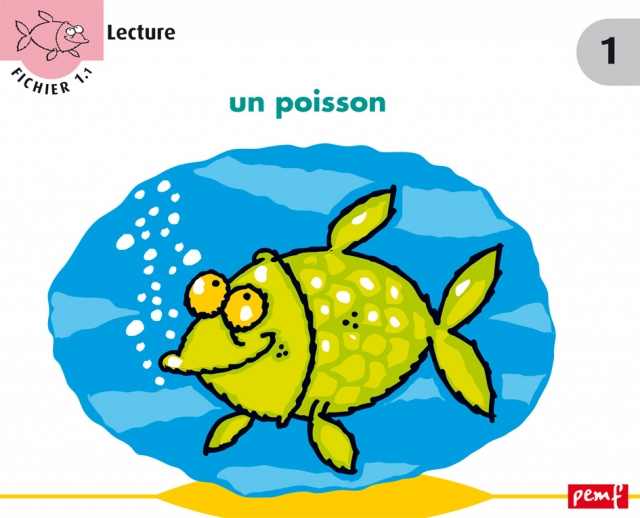
\includegraphics[width=7cm]{img/GSCP_f1recto.jpg}
   \end{minipage}  
   \begin{minipage}[c]{.46\linewidth}
      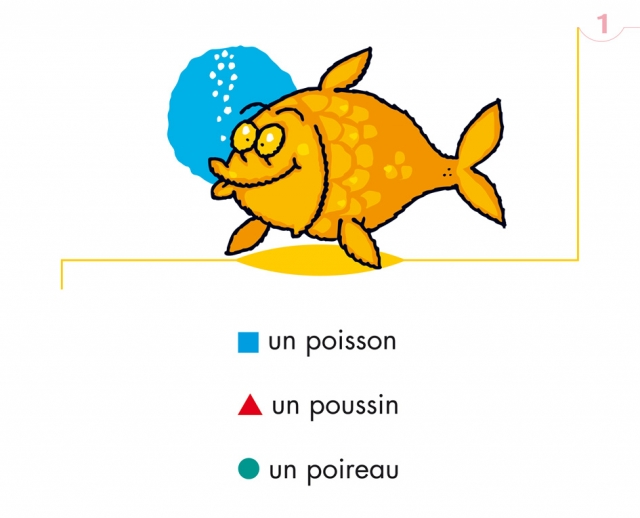
\includegraphics[width=7cm]{img/GSCP_f1verso.jpg}
   \end{minipage}
\end{figure}
\vline
\vline
\begin{figure}[h]
   \begin{minipage}[c]{.46\linewidth}
      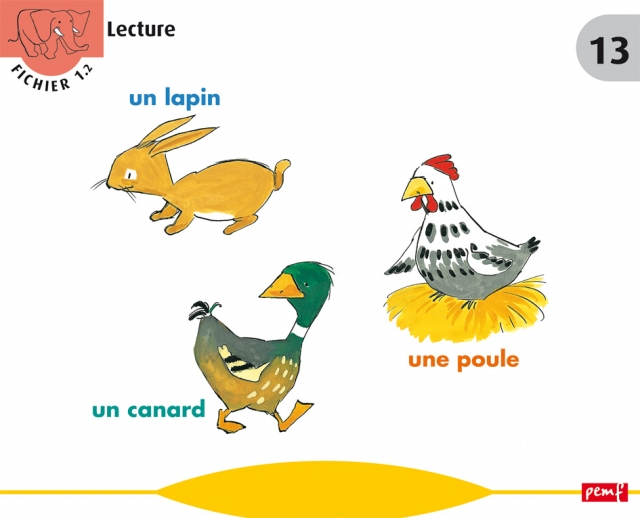
\includegraphics[width=7cm]{img/CP_niv2_f13recto.jpg}
   \end{minipage}  
   \begin{minipage}[c]{.46\linewidth}
      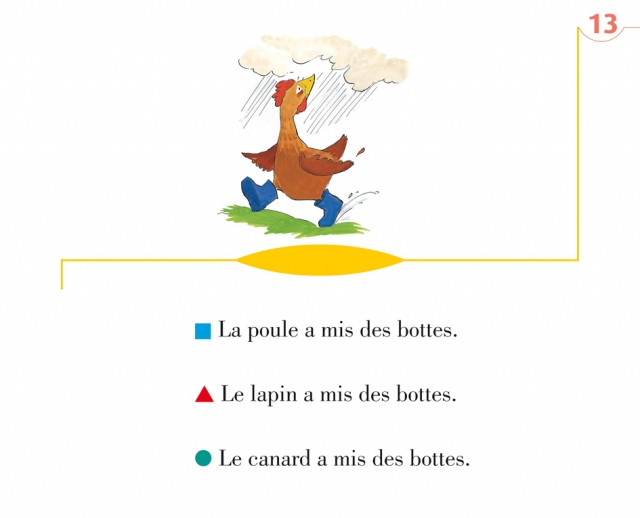
\includegraphics[width=7cm]{img/CP_niv2_f13verso.jpg}
   \end{minipage}
\end{figure}
\vline
\vline
\begin{figure}[h]
   \begin{minipage}[c]{.46\linewidth}
      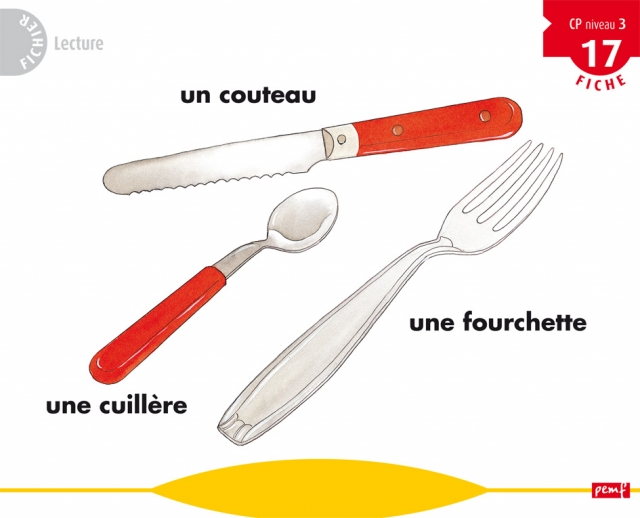
\includegraphics[width=7cm]{img/CP_niv3_f17recto.jpg}
   \end{minipage}  
   \begin{minipage}[c]{.46\linewidth}
      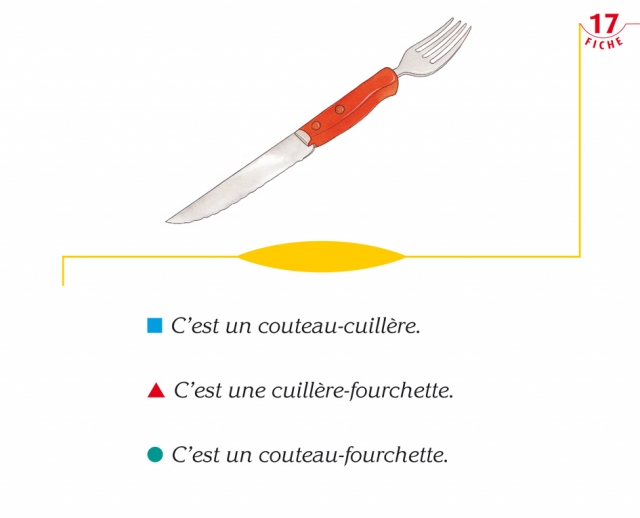
\includegraphics[width=7cm]{img/CP_niv3_f17verso.jpg}
   \end{minipage}
\end{figure}
\end{center}

\newpage
\section{VOB du cycle inférieur \label{listeVob}}
Voici la liste des mots devant être connus et maîtrisés par les enfants, téléchargée depuis \url{http://www.enseignons.be/upload/fondamental/francais/190607071618vob-degre-inferieur.pdf} le 26 janvier 2015.
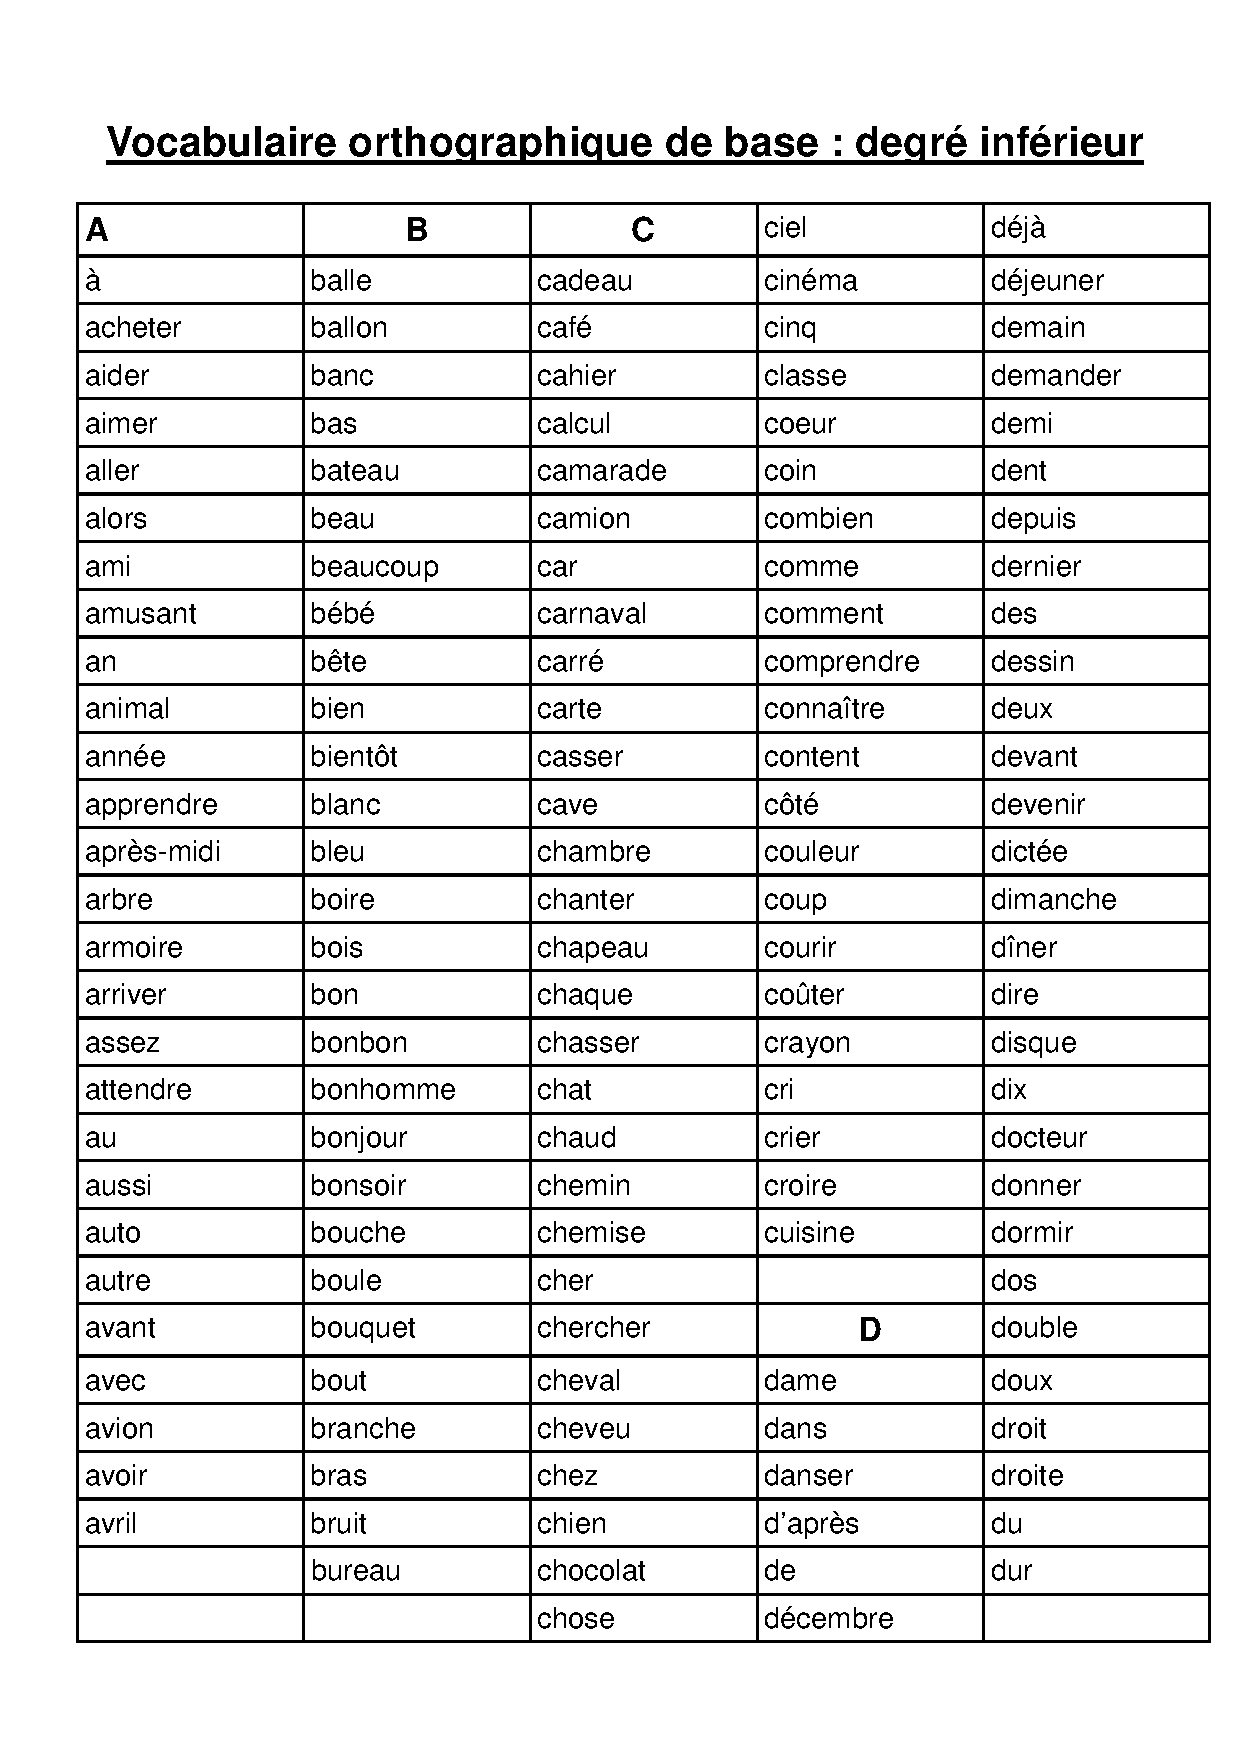
\includepdf[pages={1-4},scale=.9,pagecommand={}]{190607071618vob-degre-inferieur.pdf}


\end{document}